%===============Manual by J. Vermoesen=============================
\documentclass[11pt, a4paper]{article}
\usepackage[dutch]{babel}
%\usepackage{datetime}
%\usepackage[utf8]{inputenc}
%\usepackage[T1]{fontenc}
\usepackage{times}
\usepackage{graphicx}\graphicspath{{../gfx/}}
\usepackage[margin=1in]{geometry}
\usepackage[onehalfspacing]{setspace}
\usepackage{caption,subcaption}
\captionsetup{font={small, stretch=1}}
\usepackage[colorlinks]{hyperref}
\usepackage{cleveref}
\usepackage{biblatex}
\usepackage{csquotes}
\addbibresource{mybib.bib}
\usepackage{pdfpages}
%==================================================================

\title{\vskip-2.5cm Creditors Direct Debit APP\vskip-5mm}
\author{
  Jos Vermoesen -
  \href{https://vsoft.be}{Vsoft Belgium}}
\date{\today}

\begin{document}

\maketitle\hrule

\tableofcontents

\section{Europese domiciliëring}
  \label{sec:intro}
  In het kader van de invoering van SEPA, werden er 3 producten ontwikkeld:

  \begin{itemize}
    \item
      De Europese domiciliëring
    \item
    De Europese overschrijving
    \item
    De betaalkaart
  \end{itemize}
  Deze handleiding beperkt zich binnen de Europese domiciliëring tot de
  functionaliteit beschikbaar voor de ondernemingen (Creditors Direct
  Debit).

  \subsection{De werking van CDD}\label{sec:howto}
  Met Creditors Direct Debit kan een schuldeiser (creditor) de openstaande
  facturen van zijn klanten (debtors) in euro innen in alle landen van de
  SEPA-zone mits er een geldig mandaat bestaat. Door ondertekening van het
  mandaat geeft de debtor immers de toestemming aan de creditor om zijn
  rekening te laten debiteren. \Cref{fig:flow}

  \begin{enumerate}
    \item
    De debtor geeft een ondertekend mandaat aan de creditor om zijn rekening
    automatisch te laten debiteren.
    \item
    De creditor stuurt ter informatie een pre-notificatie naar de debtor
    (bv. een factuur).
    \item
    De creditor stuurt zijn invorderingen met mandaatgegevens aan zijn bank.
    Hij neemt het initiatief om één of meerdere inningen via zijn bank aan
    te bieden aan de bank van de debtor.
    \item
    De bank van de creditor stuurt via een interbancair uitwisselingssysteem
    (Clearing Settlement Mechanism of CSM) de bestanden door aan bank van de
    debtor.
    \item
    De bank van de debtor debiteert de rekening van de debtor.
  \end{enumerate}

  \subsection{Afbeeldingen}
  \begin{itemize}
    \item
      \Cref{fig:flow} geeft stroomschema van prille aanvang (ondertekening
      mandaat) tot aan de uitvoering van de verrichting.
    \item
    \Cref{fig:subfigs cap}
    Mo vent toch!
  \end{itemize}

  \begin{figure}
    \centering
  	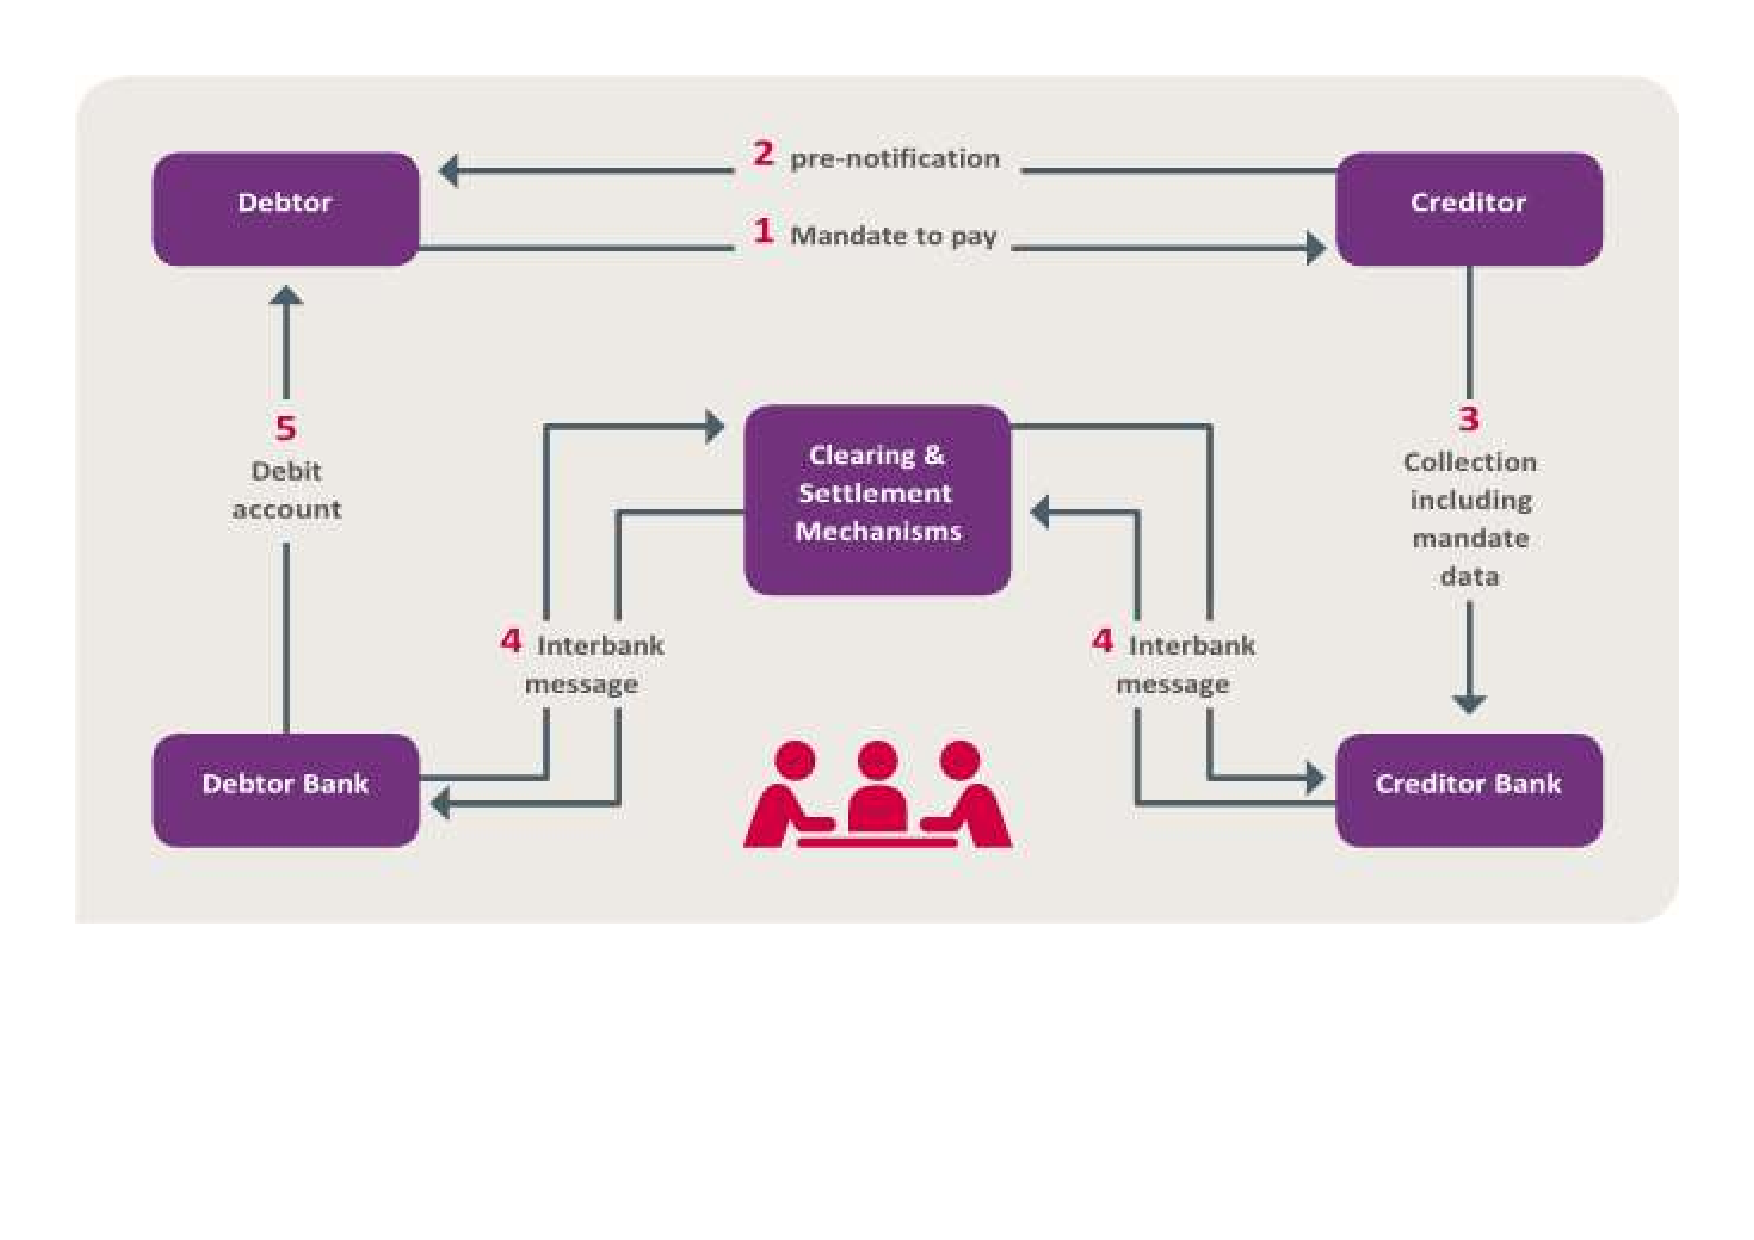
\includegraphics[width=\linewidth]{1-2-3-4-5}
    \caption{Stroomschema van een domiciliëring}
    \label{fig:flow}
  \end{figure}

  \begin{figure}
  	\centering
  	\begin{subfigure}[b]{0.45\linewidth}
		  \centering
		  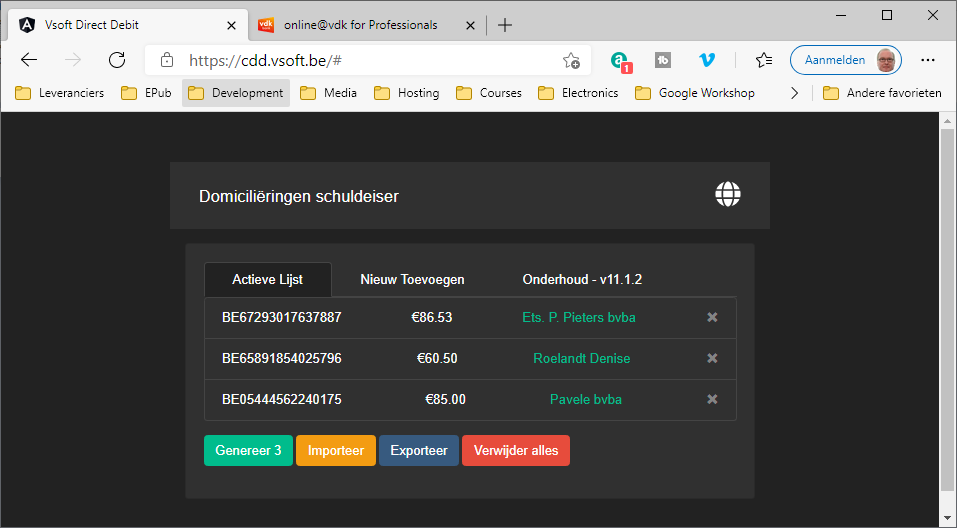
\includegraphics[width=\linewidth]{cddscreen}
		  \caption{}
		  \label{fig:cdd}
	  \end{subfigure}
	  ~
	  \begin{subfigure}[b]{0.45\linewidth}
  		\centering
		  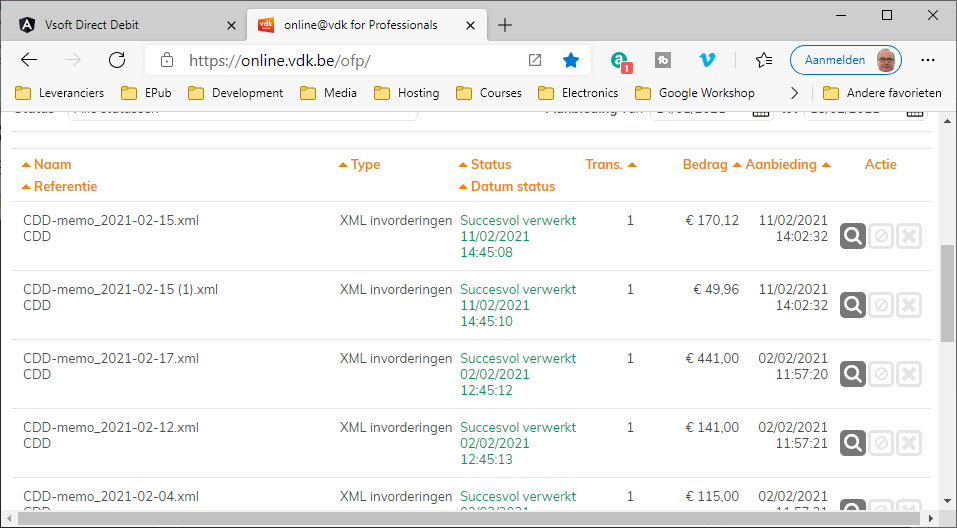
\includegraphics[width=\linewidth]{vdkscreen}
		  \caption{}
		  \label{fig:vdk}
	  \end{subfigure}
	  \caption{
      Voorbeeld van afbeeldingen naast elkaar. (a) Schermafdruk van de CDD
      app en (b) Schermafdruk van VDK app}
	  \label{fig:subfigs cap}
  \end{figure}

%\paragraph{Paragraph tile.}
%According to his explanation, a strictly controlled test execution with a
%sensibility for the subjectivity and susceptibility of outcomes due to the
%nature of man is necessary.

\section{Naslagwerken}\label{sec:lit}
Op de website van Febelfin vindt U de CDD XML handleiding \cite{febelfincdd}
alsook andere uitwisselingsstandaarden voor de ondernemer.

\section{Besluiten}\label{sec:conc}
Conclusions show readers the value of your completely developed argument or
thoroughly answered question. Consider the conclusion from the reader's
perspective. At the end of a paper, a reader wants to know how to benefit
from the work you accomplished in your paper.

\section{Ondersteuning}

\href{https://www.wikibooks.org}{wikibooks home}

\small\singlespacing

\printbibliography

\appendix
\includepdf[pages=-, pagecommand={\thispagestyle{plain}},
addtotoc={1, section, 2, XML voorbeeld, app:febelfin}
]{external-docs/{cdd-p48-50}}

\includepdf[pages=-, pagecommand={\thispagestyle{plain}},
addtotoc={1, section, 2, MANDAAT voorbeeld, app:rvmandaat}
]{external-docs/{cdd-mandate-nl}}

\end{document}
